\documentclass[tikz,border=5pt]{standalone}
\usepackage{amsmath}
\usetikzlibrary{positioning,arrows.meta}
\usepackage{ifthen}

\begin{document}
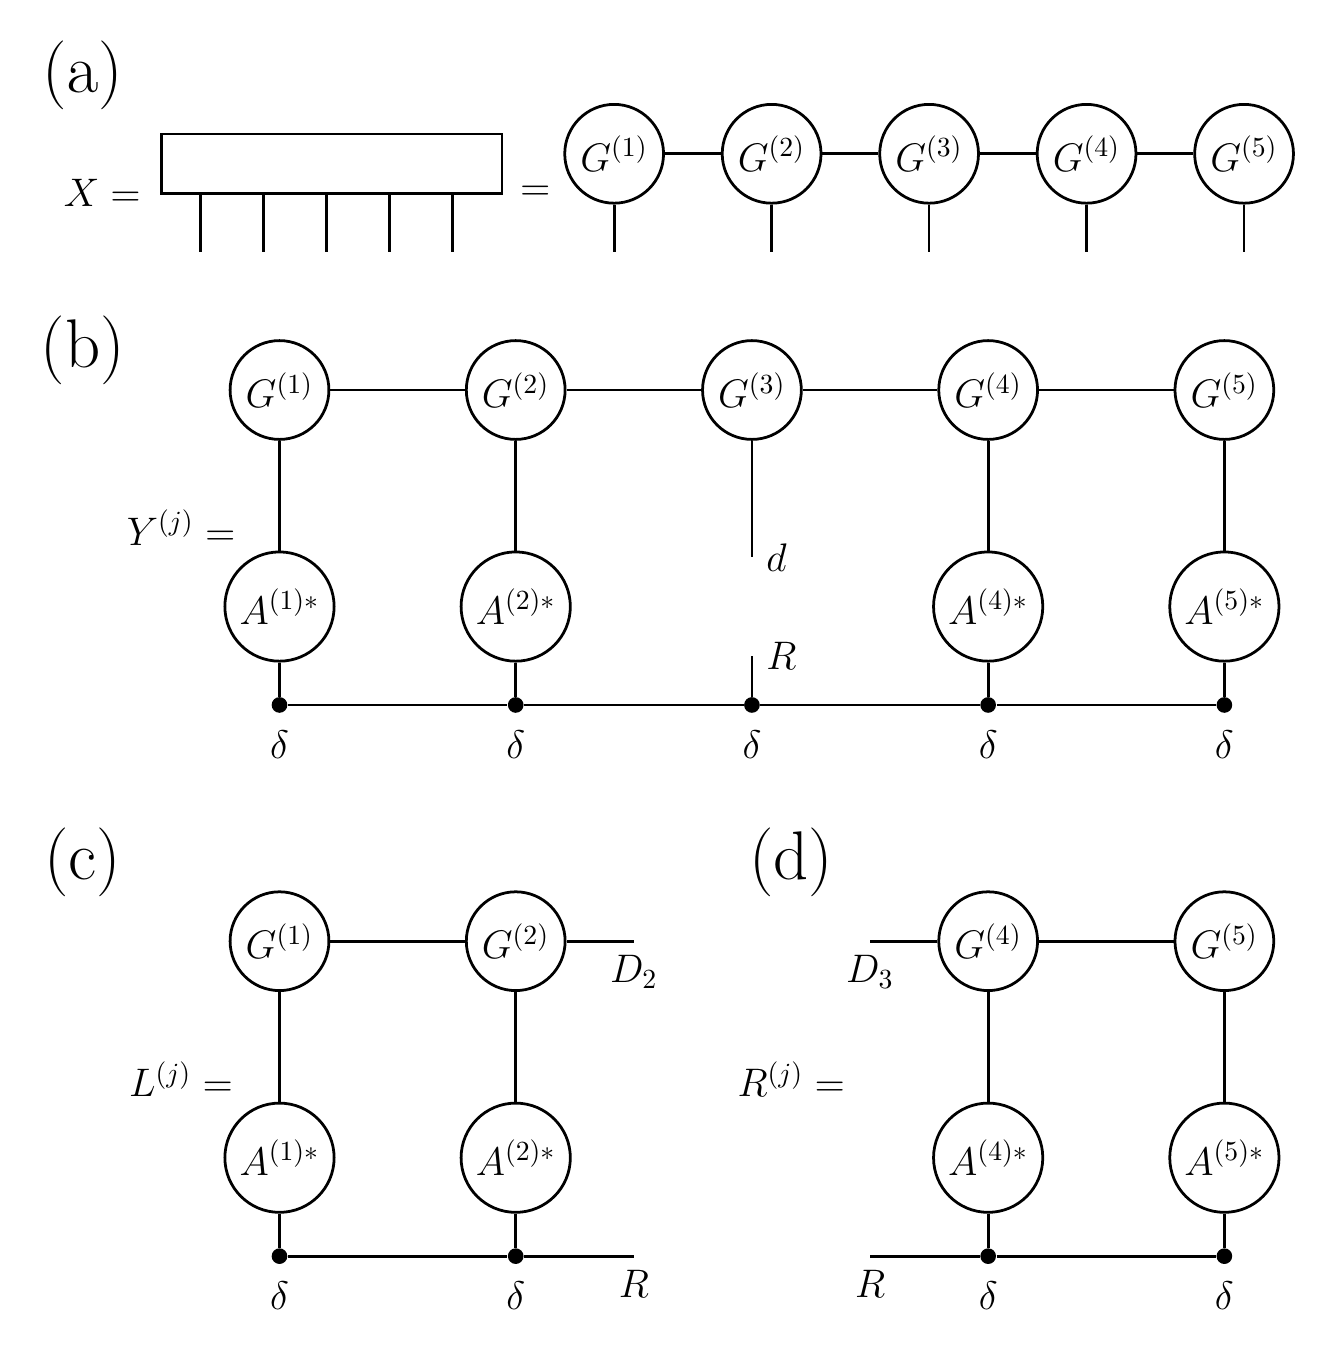
\begin{tikzpicture}[
  node/.style={circle,draw,inner sep=3pt,line width=1pt},
  dot/.style={circle,fill,inner sep=2pt},
  level distance=1.2cm,
  sibling distance=1.6cm
]

\Large

% (a)
\node at (-4.5,0.5) {\Huge{(a)}};
\node at (-4.25,-1)  {$X = $};
\draw[line width=1pt] (-3.5,-0.25) rectangle (0.825,-1);
\foreach \i in {0,1,2,3,4} {
  \draw[line width=1pt] (-3+\i*0.8,-1) -- ++(0,-0.75);
}
\node at (1.25,-1) {$=$};
\foreach \i/\x in {1/0,2/2,3/4,4/6,5/8} {
  \node[node] (G\i) at (2.25+\x,-0.5) {$G^{(\i)}$};
}
\foreach \i/\j in {1/2,2/3,3/4,4/5} {
  \draw[line width=1pt] (G\i) -- (G\j);
}
\foreach \i in {1,2,3,4,5} {
  \draw[line width=1pt] (G\i) -- ++(0,-1.25) node[below]{};
}

% (b)
\node at (-4.5,-3) {\Huge{(b)}};
\node at (-3.25,-5.25)  {$Y^{(j)} = $};
\foreach \i/\x in {1/0,2/2,3/4,4/6,5/8} {
  \node[node] (G\i) at (-2.0+\x*1.5,-3.5) {$G^{(\i)}$};
  \ifthenelse{\i=3}{
    \node (A\i) at (-2.0+\x*1.5,-6.25) {};
  }{
    \node[node] (A\i) at (-2.0+\x*1.5,-6.25) {$A^{(\i)*}$};
  }
  \node[dot]  (d\i) at (-2.0+\x*1.5,-7.5) {};
  \node at (-2.0+\x*1.5,-8) {$\delta$};
  \ifthenelse{\i=3}{
    \draw[line width=1pt] (G\i) -- ++(0,-2.125) node[right]{$d$};
    \draw[line width=1pt] (d\i) -- ++(0,0.625) node[right]{$R$};
  }{
    \draw[line width=1pt] (G\i) -- (A\i) -- (d\i);
  }
}
\draw[line width=1pt]
      (G1) -- node[above]{} (G2)
      (G2) -- node[above]{} (G3)
      (G3) -- node[above]{} (G4)
      (G4) -- node[above]{} (G5);
\draw[line width=1pt]
      (d1) -- node[below]{} (d2)
      (d2) -- node[below]{} (d3)
      (d3) -- node[below]{} (d4)
      (d4) -- node[below]{} (d5);

% (c)
\node at (-4.5,-9.5) {\Huge{(c)}};
\node at (-3.25,-12.25)  {$L^{(j)} = $};
%\foreach \i/\x in {1/0,2/2,3/4,4/6,5/8} {
\foreach \i/\x in {1/0,2/2} {
  \node[node] (GL\i) at (-2.0+\x*1.5,-10.5) {$G^{(\i)}$};
  \ifthenelse{\i=3}{
    \node (AL\i) at (-2.0+\x*1.5,-13.25) {};
  }{
    \node[node] (AL\i) at (-2.0+\x*1.5,-13.25) {$A^{(\i)*}$};
  }
  \node[dot]  (dL\i) at (-2.0+\x*1.5,-14.5) {};
  \node at (-2.0+\x*1.5,-15) {$\delta$};
  \ifthenelse{\i=3}{
    \draw[line width=1pt] (GL\i) -- ++(0,-2.125) node[right]{$d$};
    \draw[line width=1pt] (dL\i) -- ++(0,0.625) node[right]{$R$};
  }{
    \draw[line width=1pt] (GL\i) -- (AL\i) -- (dL\i);
  }
}
\draw[line width=1pt]
      (GL1) -- node[above]{} (GL2);
%      (GL2) -- node[above]{} (GL3)
%      (GL3) -- node[above]{} (GL4)
%      (GL4) -- node[above]{} (GL5);
\draw[line width=1pt]
      (dL1) -- node[below]{} (dL2);
%      (dL2) -- node[below]{} (dL3)
%      (dL3) -- node[below]{} (dL4)
%      (dL4) -- node[below]{} (dL5);
\draw[line width=1pt] (GL2) -- ++(1.5,0) node[below]{$D_2$};
\draw[line width=1pt] (dL2) -- ++(1.5,0) node[below]{$R$};

% (d)
\node at (9.00-4.5,-9.5) {\Huge{(d)}};
\node at (7.75-3.25,-12.25)  {$R^{(j)} = $};
%\foreach \i/\x in {1/0,2/2,3/4,4/6,5/8} {
\foreach \i/\x in {4/6,5/8} {
  \node[node] (GL\i) at (-2.0+\x*1.5,-10.5) {$G^{(\i)}$};
  \ifthenelse{\i=3}{
    \node (AL\i) at (-2.0+\x*1.5,-13.25) {};
  }{
    \node[node] (AL\i) at (-2.0+\x*1.5,-13.25) {$A^{(\i)*}$};
  }
  \node[dot]  (dL\i) at (-2.0+\x*1.5,-14.5) {};
  \node at (-2.0+\x*1.5,-15) {$\delta$};
  \ifthenelse{\i=3}{
    \draw[line width=1pt] (GL\i) -- ++(0,-2.125) node[right]{$d$};
    \draw[line width=1pt] (dL\i) -- ++(0,0.625) node[right]{$R$};
  }{
    \draw[line width=1pt] (GL\i) -- (AL\i) -- (dL\i);
  }
}
\draw[line width=1pt]
%      (GL1) -- node[above]{} (GL2)
%      (GL2) -- node[above]{} (GL3)
%      (GL3) -- node[above]{} (GL4)
      (GL4) -- node[above]{} (GL5);
\draw[line width=1pt]
%      (dL1) -- node[below]{} (dL2)
%      (dL2) -- node[below]{} (dL3)
%      (dL3) -- node[below]{} (dL4)
      (dL4) -- node[below]{} (dL5);
\draw[line width=1pt] (GL4) -- ++(-1.5,0) node[below]{$D_3$};
\draw[line width=1pt] (dL4) -- ++(-1.5,0) node[below]{$R$};


\end{tikzpicture}
\end{document}

